\documentclass[12pt,]{article}
\usepackage{lmodern}
\usepackage{amssymb,amsmath}
\usepackage{ifxetex,ifluatex}
\usepackage{fixltx2e} % provides \textsubscript
\ifnum 0\ifxetex 1\fi\ifluatex 1\fi=0 % if pdftex
  \usepackage[T1]{fontenc}
  \usepackage[utf8]{inputenc}
\else % if luatex or xelatex
  \ifxetex
    \usepackage{mathspec}
  \else
    \usepackage{fontspec}
  \fi
  \defaultfontfeatures{Ligatures=TeX,Scale=MatchLowercase}
    \setmainfont[]{Times New Roman}
\fi
% use upquote if available, for straight quotes in verbatim environments
\IfFileExists{upquote.sty}{\usepackage{upquote}}{}
% use microtype if available
\IfFileExists{microtype.sty}{%
\usepackage{microtype}
\UseMicrotypeSet[protrusion]{basicmath} % disable protrusion for tt fonts
}{}
\usepackage[margin=2.54cm]{geometry}
\usepackage{hyperref}
\hypersetup{unicode=true,
            pdftitle={Trends in Alternative Daily Cover in California},
            pdfauthor={Sarah Ko},
            pdfborder={0 0 0},
            breaklinks=true}
\urlstyle{same}  % don't use monospace font for urls
\usepackage{color}
\usepackage{fancyvrb}
\newcommand{\VerbBar}{|}
\newcommand{\VERB}{\Verb[commandchars=\\\{\}]}
\DefineVerbatimEnvironment{Highlighting}{Verbatim}{commandchars=\\\{\}}
% Add ',fontsize=\small' for more characters per line
\usepackage{framed}
\definecolor{shadecolor}{RGB}{248,248,248}
\newenvironment{Shaded}{\begin{snugshade}}{\end{snugshade}}
\newcommand{\KeywordTok}[1]{\textcolor[rgb]{0.13,0.29,0.53}{\textbf{#1}}}
\newcommand{\DataTypeTok}[1]{\textcolor[rgb]{0.13,0.29,0.53}{#1}}
\newcommand{\DecValTok}[1]{\textcolor[rgb]{0.00,0.00,0.81}{#1}}
\newcommand{\BaseNTok}[1]{\textcolor[rgb]{0.00,0.00,0.81}{#1}}
\newcommand{\FloatTok}[1]{\textcolor[rgb]{0.00,0.00,0.81}{#1}}
\newcommand{\ConstantTok}[1]{\textcolor[rgb]{0.00,0.00,0.00}{#1}}
\newcommand{\CharTok}[1]{\textcolor[rgb]{0.31,0.60,0.02}{#1}}
\newcommand{\SpecialCharTok}[1]{\textcolor[rgb]{0.00,0.00,0.00}{#1}}
\newcommand{\StringTok}[1]{\textcolor[rgb]{0.31,0.60,0.02}{#1}}
\newcommand{\VerbatimStringTok}[1]{\textcolor[rgb]{0.31,0.60,0.02}{#1}}
\newcommand{\SpecialStringTok}[1]{\textcolor[rgb]{0.31,0.60,0.02}{#1}}
\newcommand{\ImportTok}[1]{#1}
\newcommand{\CommentTok}[1]{\textcolor[rgb]{0.56,0.35,0.01}{\textit{#1}}}
\newcommand{\DocumentationTok}[1]{\textcolor[rgb]{0.56,0.35,0.01}{\textbf{\textit{#1}}}}
\newcommand{\AnnotationTok}[1]{\textcolor[rgb]{0.56,0.35,0.01}{\textbf{\textit{#1}}}}
\newcommand{\CommentVarTok}[1]{\textcolor[rgb]{0.56,0.35,0.01}{\textbf{\textit{#1}}}}
\newcommand{\OtherTok}[1]{\textcolor[rgb]{0.56,0.35,0.01}{#1}}
\newcommand{\FunctionTok}[1]{\textcolor[rgb]{0.00,0.00,0.00}{#1}}
\newcommand{\VariableTok}[1]{\textcolor[rgb]{0.00,0.00,0.00}{#1}}
\newcommand{\ControlFlowTok}[1]{\textcolor[rgb]{0.13,0.29,0.53}{\textbf{#1}}}
\newcommand{\OperatorTok}[1]{\textcolor[rgb]{0.81,0.36,0.00}{\textbf{#1}}}
\newcommand{\BuiltInTok}[1]{#1}
\newcommand{\ExtensionTok}[1]{#1}
\newcommand{\PreprocessorTok}[1]{\textcolor[rgb]{0.56,0.35,0.01}{\textit{#1}}}
\newcommand{\AttributeTok}[1]{\textcolor[rgb]{0.77,0.63,0.00}{#1}}
\newcommand{\RegionMarkerTok}[1]{#1}
\newcommand{\InformationTok}[1]{\textcolor[rgb]{0.56,0.35,0.01}{\textbf{\textit{#1}}}}
\newcommand{\WarningTok}[1]{\textcolor[rgb]{0.56,0.35,0.01}{\textbf{\textit{#1}}}}
\newcommand{\AlertTok}[1]{\textcolor[rgb]{0.94,0.16,0.16}{#1}}
\newcommand{\ErrorTok}[1]{\textcolor[rgb]{0.64,0.00,0.00}{\textbf{#1}}}
\newcommand{\NormalTok}[1]{#1}
\usepackage{graphicx,grffile}
\makeatletter
\def\maxwidth{\ifdim\Gin@nat@width>\linewidth\linewidth\else\Gin@nat@width\fi}
\def\maxheight{\ifdim\Gin@nat@height>\textheight\textheight\else\Gin@nat@height\fi}
\makeatother
% Scale images if necessary, so that they will not overflow the page
% margins by default, and it is still possible to overwrite the defaults
% using explicit options in \includegraphics[width, height, ...]{}
\setkeys{Gin}{width=\maxwidth,height=\maxheight,keepaspectratio}
\IfFileExists{parskip.sty}{%
\usepackage{parskip}
}{% else
\setlength{\parindent}{0pt}
\setlength{\parskip}{6pt plus 2pt minus 1pt}
}
\setlength{\emergencystretch}{3em}  % prevent overfull lines
\providecommand{\tightlist}{%
  \setlength{\itemsep}{0pt}\setlength{\parskip}{0pt}}
\setcounter{secnumdepth}{5}
% Redefines (sub)paragraphs to behave more like sections
\ifx\paragraph\undefined\else
\let\oldparagraph\paragraph
\renewcommand{\paragraph}[1]{\oldparagraph{#1}\mbox{}}
\fi
\ifx\subparagraph\undefined\else
\let\oldsubparagraph\subparagraph
\renewcommand{\subparagraph}[1]{\oldsubparagraph{#1}\mbox{}}
\fi

%%% Use protect on footnotes to avoid problems with footnotes in titles
\let\rmarkdownfootnote\footnote%
\def\footnote{\protect\rmarkdownfootnote}

%%% Change title format to be more compact
\usepackage{titling}

% Create subtitle command for use in maketitle
\providecommand{\subtitle}[1]{
  \posttitle{
    \begin{center}\large#1\end{center}
    }
}

\setlength{\droptitle}{-2em}

  \title{Trends in Alternative Daily Cover in California}
    \pretitle{\vspace{\droptitle}\centering\huge}
  \posttitle{\par}
  \subtitle{\url{https://github.com/sarahko7/ADC_Analysis}}
  \author{Sarah Ko}
    \preauthor{\centering\large\emph}
  \postauthor{\par}
    \date{}
    \predate{}\postdate{}
  
\usepackage{booktabs}
\usepackage{longtable}
\usepackage{array}
\usepackage{multirow}
\usepackage{wrapfig}
\usepackage{float}
\usepackage{colortbl}
\usepackage{pdflscape}
\usepackage{tabu}
\usepackage{threeparttable}
\usepackage{threeparttablex}
\usepackage[normalem]{ulem}
\usepackage{makecell}
\usepackage{xcolor}

\begin{document}
\maketitle
\begin{abstract}
Daily cover (DC) is the material, often soil, that is spread over
garbage layers in a landfill. DC serves to reduce odor, slow
infiltration by water, prevent garbage from being blown away, and deter
pests like small mammals and birds. The state of California defines an
alternative daily cover (ADC) as a material other than soil. This study
uses the data from CalRecycle to investigate trends in state-wide use of
alternative daily cover. When analyzing trends in reporting quarter,
statistical tests found that quantities in each quarter are not
significantly different from one another. In a second test, quarterly
ADC quantities were modeled as a function of time - the linear model
((Quarterly Quantity = 73.14*Date - 190264.58)) was a moderate fit,
explaining \textasciitilde{}44\% of the variation. However, the Loess
regression appears to be a much better fit visually. For construction \&
demolition ADC specifically, tests detected 2 changepoints in the
quantities over time - one around 2008-02-14, and another around
2015-02-14. It is notable though that these changepoints do not seem to
be represented strongly in the visual depiction of the data. Findings
from this analysis can be used to help rule makers and policymakers make
more informed decisions regarding circular economy standards and
regulations.
\end{abstract}

\newpage

\tableofcontents 

\newpage

\newpage

\listoftables 

Table 1: Summary of Data Structure

Table 2: Summary statistics of ADC, separated by type

Table 3: Summary statistics of ADC, separated by year

\newpage

\listoffigures 

Figure 1: 2017 Quantities of ADC, separated by type

Figure 2: Quarterly quantities of ADC are grouped for each year. The
data is displayed by ADC type

Figure 3: Quantities of ADC are grouped by the reporting quarter. The
report year is classified by color, and the ADC type is classified by
icon shape

Figure 4: Quantities of ADC are grouped by quarter. The height of the
bar described the spread of the data, a the width of the bar describes
the number of records at each quantity

Figure 5: Quarterly quantities of ADC are plotted by time, and fit with
the equation y = 73.14*time -190264.58

Figure 6: Quarterly quantities of ADC are plotted by time, and fit with
a Loess Regression

Figure 7: Quarterly quantities of Construction \& Demolition ADC are
plotted by time, and the 2 changepoints are marked with dotted lines

\newpage

\section{Research Question and
Rationale}\label{research-question-and-rationale}

As described by CalRecycle, alternative daily cover (ADC) is a cover
other than `earthen' material that is spread over the active face of a
municipal solid waste landfill at the end of each operating day. Certain
regions in California can claim materials used for ADC as diverted from
landfill, which is an important characteristic for certifications that
are promoting circular economy concepts. As circular economy related
rules and regulations change over time, the quantities of ADC may see
changes as well. Construction \& demolition waste is of particular
interest because of a particular constituent - gypsum wallboard. Under
the anerobic decomposition of a landfill, this material forms hydrogen
sulfide gas, which is not only highly toxic, but is also corrosive to
the methane collection equipment used in landfills.

This analysis has 3 main research questions:

\begin{enumerate}
\def\labelenumi{\arabic{enumi})}
\item
  For all ADC types combined, is there a significant difference in the
  quantity of ADC used in each reporting quarter?
\item
  For all ADC types combined, can the quarterly quantities be modeled as
  a function of time?
\item
  For construction \& demolition ADC specifically, have there been
  changepoints in the quantities over time?
\end{enumerate}

The first research question is an important component of understanding
the trends of ADC over yearly seasons. This could signify an oversupply
of ADC in a particular season (e.g.~green material may be more plentiful
in the summer), or an undersupply of earthen material. The second
research question would be helpful in making predictions of future use
of ADC. If the model predicts that the use of ADC is growing, this could
be due to the influence of policies surrounding landfill diversion
standards. The third research question looks at C\&D ADC specifically -
since this type of ADC is highly related to new and retrofit building
construction, changepoints in this data could be related to trends in
construction related sustainability standards. The dataset used to
answer these questions is from the CalRecycle website - it includes
quarterly information for ADC, split up by type. This allows for
timeseries analyses, as well as analyses specific to certain waste
types.

References:

\url{https://www.calrecycle.ca.gov/lgcentral/basics/adcbasic}

\url{http://www.newmoa.org/solidwaste/projects/gypsum.cfm}

\newpage

\section{Dataset Information}\label{dataset-information}

The data used for this analysis was taken from CalRecycle - the database
of the California Department of Resources Recycling and Recovery. This
department is a part of the California Environmental Protection Agency.
For more information about CalRecycle, see the `About Us' section of the
website: \url{https://www.calrecycle.ca.gov/AboutUs/}

The specific data used for this analysis is found on the page `Statewide
Alternative Daily Cover (ADC) by Material Type':
\url{https://www2.calrecycle.ca.gov/LGCentral/DisposalReporting/Statewide/ADCByMaterialType}.
To extract the information, the data was exported to excel, then saved
as a CSV file. The data for this analysis was extracted on 2009-04-06
(April 6, 2019).

ADC quantities are classified by 10 material types: Ash, Auto Shredder
Waste, Compost, Construction \& Demolition Waste, Contaminated Sediment,
Green Material, Mixed, Other, Sludge, and Tires. A more detailed
description of the data structure is found in Table 1. Classification of
ADC into the full 10 categories was started in 1998. Prior to 1998, most
of the ADC was categorized as `Other'. The oldest datapoint in this
record is Q1, 1995. The newest datapoint is Q4, 2017.

The quantities of ADC in this analysis are in units of U.S. tons, which
is equivalent to 2000 lbs.

Table 1: Summary of Data Structure

\begin{table}[H]
\centering
\begin{tabular}{l|l}
\hline
\textbf{Column Name} & \textbf{Data Description}\\
\hline
Report Year & Year that the ADC was used\\
\hline
Report Quarter & Quarter that the ADC was used\\
\hline
Ash & Ash and cement kiln dust materials\\
\hline
Auto Shredder Waste & Treated auto shredder waste\\
\hline
Construction and Demolition Waste & Processed construction and demolition wastes and materials\\
\hline
Compost & Compost materials\\
\hline
Contaminated Sediment & Contaminated sediment, dredge spoils, foundry sands\\
\hline
Green Material & Processed green material\\
\hline
Mixed & Mixtures of the other categories\\
\hline
Other & Before 1998, most ADC was classified in this category\\
\hline
Tires & Shredded tires\\
\hline
Sludge & Sludge and sludge-derived materials\\
\hline
Total & Sum of the columns Ash:Sludge\\
\hline
\end{tabular}
\end{table}

\newpage

\section{Exploratory Data Analysis and
Wrangling}\label{exploratory-data-analysis-and-wrangling}

\subsection{Data Wrangling}\label{data-wrangling}

The first part of wrangling the data was creating a dataset with only
the years 1998-2017. The years before 1998 were removed because most of
the ADC in that time was classified as `Other'. If this data were
included in analyses considering ADC types, the data from these years
would make this category appear artificially large.

After reviewing the dataset, the second part of the wrangling process
was to `tidy' the data. The function `gather' was used to rearrange the
data under each type column into 2 new columns: ADC Type, and Quantity.
This was done to facilitate visualization and statistical analyses
later.

\begin{Shaded}
\begin{Highlighting}[]
\CommentTok{# per the CalRecycle website, segregation into ADC types started in 1998}
\CommentTok{# therefore, for the analysis, remove data from before 1998}
\KeywordTok{class}\NormalTok{(ADC_raw}\OperatorTok{$}\NormalTok{Report.Year)}
\end{Highlighting}
\end{Shaded}

\begin{verbatim}
## [1] "integer"
\end{verbatim}

\begin{Shaded}
\begin{Highlighting}[]
\NormalTok{ADC_data <-}\StringTok{ }\KeywordTok{filter}\NormalTok{(ADC_raw, Report.Year }\OperatorTok{>=}\StringTok{ }\DecValTok{1998}\NormalTok{)}
\KeywordTok{dim}\NormalTok{(ADC_data)}
\end{Highlighting}
\end{Shaded}

\begin{verbatim}
## [1] 80 13
\end{verbatim}

\begin{Shaded}
\begin{Highlighting}[]
\CommentTok{# explore new dataset}
\KeywordTok{head}\NormalTok{(ADC_data)}
\end{Highlighting}
\end{Shaded}

\begin{verbatim}
##   Report.Year Report.Quarter      Ash Auto.Shredder.Waste
## 1        2017              1 32511.83            153270.6
## 2        2017              2 37294.78            159759.7
## 3        2017              3 33349.25            153342.6
## 4        2017              4 22248.85            123203.5
## 5        2016              1 31423.40            123193.3
## 6        2016              2 45504.45            126040.9
##   Construction.and.Demolition.Waste  Compost Contaminated.Sediment
## 1                          173548.6  6128.89               3396.36
## 2                          199486.8  2746.22               7585.58
## 3                          164028.4  1796.97               4280.92
## 4                          198901.7 15993.13               2979.12
## 5                          160446.5 15681.63              20203.18
## 6                          144982.9 42215.62              18089.73
##   Green.Material    Mixed    Other   Tires    Sludge    Total
## 1       380686.2     0.00 71983.68 3771.40  68063.34 893360.9
## 2       401034.3  1516.12 71066.46 5066.35  65585.25 951141.6
## 3       362474.4 10891.73 78980.55 5323.75  79967.05 894435.6
## 4       347204.0  7964.83 56849.63 4575.75 141423.92 921344.5
## 5       334512.7 12756.90 82081.97 3402.03  83424.85 867126.5
## 6       310959.5 17946.71 75803.52 3616.26  72882.61 858042.2
\end{verbatim}

\begin{Shaded}
\begin{Highlighting}[]
\KeywordTok{tail}\NormalTok{(ADC_data)}
\end{Highlighting}
\end{Shaded}

\begin{verbatim}
##    Report.Year Report.Quarter     Ash Auto.Shredder.Waste
## 75        1999              3 1578.70            69300.25
## 76        1999              4 2718.22            63910.19
## 77        1998              1 2631.85            39181.17
## 78        1998              2  878.63            49391.25
## 79        1998              3 2457.00            35573.00
## 80        1998              4 2418.00            38495.89
##    Construction.and.Demolition.Waste Compost Contaminated.Sediment
## 75                          48321.13       0                  0.00
## 76                          62057.02     381                 16.50
## 77                           2693.48       0                  0.00
## 78                           6666.70       0                  2.74
## 79                          28278.30       0                 92.17
## 80                          29591.80       0                  0.00
##    Green.Material   Mixed   Other    Tires   Sludge    Total
## 75       349276.6    0.00 4695.69  1265.82 66864.38 541302.6
## 76       360153.2    0.00 6316.72  3307.48 69058.27 567918.6
## 77       191066.3 3907.20 1008.27 14802.71 43391.12 298682.1
## 78       279191.3 3602.22 3305.93 15394.54 92416.47 450849.8
## 79       299986.8    0.00 2706.53  2943.31 99312.34 471349.4
## 80       313452.3 4130.00 3767.93   733.71 57511.25 450100.9
\end{verbatim}

\begin{Shaded}
\begin{Highlighting}[]
\CommentTok{# tidy the data by gathering the type columns}
\NormalTok{ADC_gathered <-}\StringTok{ }\KeywordTok{gather}\NormalTok{(ADC_data, }\StringTok{"Type"}\NormalTok{, }\StringTok{"Quantity"}\NormalTok{, Ash}\OperatorTok{:}\NormalTok{Sludge) }\OperatorTok
\StringTok{  }\KeywordTok{select}\NormalTok{(}\OperatorTok{-}\NormalTok{Total) }\CommentTok{# remove Total column}

\CommentTok{# save the tidy dataset}
\KeywordTok{write.csv}\NormalTok{(ADC_data, }\DataTypeTok{row.names =} \OtherTok{FALSE}\NormalTok{, }
          \DataTypeTok{file =} \StringTok{"../Processed_Data/CalRecycle_ADC_tidy_processed.csv"}\NormalTok{)}
\end{Highlighting}
\end{Shaded}

\subsection{Summary}\label{summary}

The following code is used to generate summary information about the
data. This provides a general sense of the range and spread of the data.
The `group' and `summarize' functions were used to generate this
information.

Table 2 describes the summary statistics separated by type. Green
material, construction \& demolition, and auto shredder waste are seen
to dominate the means. The sd column shows that green material has a
much larger spread in its data as compared to the other types.

Table 3 describes the summary statistics separated by year. The mean
quarterly quantities appear to peak between 2005-2008, and again in
2011.

\begin{Shaded}
\begin{Highlighting}[]
\CommentTok{# generate summary data}
\NormalTok{ADC_summary_by_type <-}\StringTok{ }\NormalTok{ADC_gathered }\OperatorTok
\StringTok{  }\KeywordTok{group_by}\NormalTok{(Type) }\OperatorTok\StringTok{ }\CommentTok{# group the data by lakename}
\StringTok{  }\KeywordTok{filter}\NormalTok{(}\OperatorTok{!}\KeywordTok{is.na}\NormalTok{(Quantity)) }\OperatorTok\StringTok{ }\CommentTok{#remove the records when there are nas Quantity}
\StringTok{  }\KeywordTok{summarise}\NormalTok{(}\DataTypeTok{MeanQuarterlyQuantity =} \KeywordTok{mean}\NormalTok{(Quantity), }
            \DataTypeTok{MinQuarterlyQuantity =} \KeywordTok{min}\NormalTok{(Quantity), }
            \DataTypeTok{MaxQuarterlyQuantity =} \KeywordTok{max}\NormalTok{(Quantity), }
            \DataTypeTok{sdQuarterlyQuantity =} \KeywordTok{sd}\NormalTok{(Quantity), }
            \DataTypeTok{medianQuarterlyQuantity =} \KeywordTok{median}\NormalTok{(Quantity))}

\NormalTok{ADC_summary_by_type_table <-}\StringTok{ }\KeywordTok{kable}\NormalTok{(ADC_summary_by_type, }
  \DataTypeTok{col.names =} \KeywordTok{c}\NormalTok{(}\StringTok{"Waste Type"}\NormalTok{, }\StringTok{"Mean Quarterly Quantity"}\NormalTok{, }\StringTok{"Min Quarterly Quantity"}\NormalTok{, }
  \StringTok{"Max Quarterly Quantity"}\NormalTok{, }\StringTok{"sd of Quarterly Quantity"}\NormalTok{, }
  \StringTok{"Median Quarterly Quantity"}\NormalTok{)) }\OperatorTok
\StringTok{  }\KeywordTok{kable_styling}\NormalTok{(}\DataTypeTok{bootstrap_options =} \KeywordTok{c}\NormalTok{(}\StringTok{"striped"}\NormalTok{, }\StringTok{"hover"}\NormalTok{, }\StringTok{"condensed"}\NormalTok{, }
                                \StringTok{"full_width = F"}\NormalTok{), }\DataTypeTok{latex_options=}\StringTok{"scale_down"}\NormalTok{) }\OperatorTok\StringTok{ }
\StringTok{  }\KeywordTok{row_spec}\NormalTok{(}\DecValTok{0}\NormalTok{, }\DataTypeTok{bold =}\NormalTok{ T)}
\end{Highlighting}
\end{Shaded}

Table 2: Summary statistics of ADC, separated by type

\begin{table}[H]
\centering
\resizebox{\linewidth}{!}{
\begin{tabular}{l|r|r|r|r|r}
\hline
\textbf{Waste Type} & \textbf{Mean Quarterly Quantity} & \textbf{Min Quarterly Quantity} & \textbf{Max Quarterly Quantity} & \textbf{sd of Quarterly Quantity} & \textbf{Median Quarterly Quantity}\\
\hline
Ash & 11304.716 & 101.00 & 108208.23 & 17860.123 & 2675.035\\
\hline
Auto.Shredder.Waste & 121864.560 & 35573.00 & 215857.61 & 39655.164 & 123356.730\\
\hline
Compost & 3451.346 & 0.00 & 42215.62 & 6437.880 & 816.520\\
\hline
Construction.and.Demolition.Waste & 122445.102 & 2693.48 & 281972.47 & 58940.701 & 125469.485\\
\hline
Contaminated.Sediment & 11632.401 & 0.00 & 102850.25 & 20862.617 & 873.295\\
\hline
Green.Material & 464016.026 & 191066.26 & 797463.76 & 137342.174 & 431369.340\\
\hline
Mixed & 6929.398 & 0.00 & 99288.87 & 12855.562 & 3618.210\\
\hline
Other & 45163.726 & 1008.27 & 149415.30 & 33034.798 & 47919.710\\
\hline
Sludge & 73697.705 & 23812.68 & 147167.22 & 23765.135 & 72039.815\\
\hline
Tires & 6544.532 & 733.71 & 29842.28 & 5735.144 & 4353.135\\
\hline
\end{tabular}}
\end{table}

\begin{Shaded}
\begin{Highlighting}[]
\NormalTok{ADC_summary_by_year <-}\StringTok{ }\NormalTok{ADC_gathered }\OperatorTok
\StringTok{  }\KeywordTok{group_by}\NormalTok{(Report.Year) }\OperatorTok\StringTok{ }\CommentTok{# group the data by year}
\StringTok{  }\KeywordTok{filter}\NormalTok{(}\OperatorTok{!}\KeywordTok{is.na}\NormalTok{(Quantity)) }\OperatorTok\StringTok{ }\CommentTok{#remove the records when there are nas Quantity}
\StringTok{  }\KeywordTok{summarise}\NormalTok{(}\DataTypeTok{MeanQuarterlyQuantity =} \KeywordTok{mean}\NormalTok{(Quantity), }
            \DataTypeTok{MinQuarterlyQuantity =} \KeywordTok{min}\NormalTok{(Quantity), }
            \DataTypeTok{MaxQuarterlyQuantity =} \KeywordTok{max}\NormalTok{(Quantity), }
            \DataTypeTok{sdQuarterlyQuantity =} \KeywordTok{sd}\NormalTok{(Quantity), }
            \DataTypeTok{medianQuarterlyQuantity =} \KeywordTok{median}\NormalTok{(Quantity))}

\NormalTok{ADC_summary_by_year_table <-}\StringTok{ }\KeywordTok{kable}\NormalTok{(ADC_summary_by_year, }
  \DataTypeTok{col.names =} \KeywordTok{c}\NormalTok{(}\StringTok{"Year"}\NormalTok{, }\StringTok{"Mean Quarterly Quantity"}\NormalTok{, }\StringTok{"Min Quarterly Quantity"}\NormalTok{, }
  \StringTok{"Max Quarterly Quantity"}\NormalTok{, }\StringTok{"sd of Quarterly Quantity"}\NormalTok{, }
  \StringTok{"Median Quarterly Quantity"}\NormalTok{)) }\OperatorTok
\StringTok{  }\KeywordTok{kable_styling}\NormalTok{(}\DataTypeTok{bootstrap_options =} \KeywordTok{c}\NormalTok{(}\StringTok{"striped"}\NormalTok{, }\StringTok{"hover"}\NormalTok{, }\StringTok{"condensed"}\NormalTok{, }
                                \StringTok{"full_width = F"}\NormalTok{), }\DataTypeTok{latex_options=}\StringTok{"scale_down"}\NormalTok{) }\OperatorTok\StringTok{ }
\StringTok{  }\KeywordTok{row_spec}\NormalTok{(}\DecValTok{0}\NormalTok{, }\DataTypeTok{bold =}\NormalTok{ T)}
\end{Highlighting}
\end{Shaded}

Table 3: Summary statistics of ADC, separated by year

\begin{table}[H]
\centering
\resizebox{\linewidth}{!}{
\begin{tabular}{r|r|r|r|r|r}
\hline
\textbf{Year} & \textbf{Mean Quarterly Quantity} & \textbf{Min Quarterly Quantity} & \textbf{Max Quarterly Quantity} & \textbf{sd of Quarterly Quantity} & \textbf{Median Quarterly Quantity}\\
\hline
1998 & 41774.55 & 0.00 & 313452.3 & 82508.86 & 3685.075\\
\hline
1999 & 54320.11 & 0.00 & 383358.8 & 103282.44 & 4657.845\\
\hline
2000 & 72004.54 & 0.00 & 437691.8 & 124324.24 & 12219.725\\
\hline
2001 & 80768.84 & 0.00 & 550962.5 & 147577.35 & 10910.315\\
\hline
2002 & 81108.82 & 0.00 & 572016.4 & 162476.47 & 8921.990\\
\hline
2003 & 86182.39 & 0.00 & 704649.9 & 178905.18 & 8734.895\\
\hline
2004 & 94959.32 & 0.00 & 680872.4 & 193691.28 & 22845.585\\
\hline
2005 & 116741.86 & 0.00 & 797463.8 & 223003.44 & 11838.200\\
\hline
2006 & 105499.79 & 0.00 & 731872.6 & 196767.51 & 19307.055\\
\hline
2007 & 98051.49 & 0.00 & 592911.4 & 169159.05 & 33313.725\\
\hline
2008 & 104818.28 & 93.00 & 587091.4 & 164134.03 & 45992.905\\
\hline
2009 & 83490.23 & 264.00 & 461620.7 & 130916.23 & 31683.365\\
\hline
2010 & 87194.48 & 21.59 & 457554.9 & 125910.72 & 36318.670\\
\hline
2011 & 103442.44 & 90.18 & 448355.7 & 128119.69 & 60689.255\\
\hline
2012 & 87318.52 & 228.26 & 445240.2 & 120284.80 & 49674.030\\
\hline
2013 & 82700.26 & 31.08 & 395495.6 & 107155.27 & 52122.570\\
\hline
2014 & 85596.00 & 0.00 & 343124.0 & 97936.53 & 57852.960\\
\hline
2015 & 87924.03 & 0.00 & 359753.1 & 105114.41 & 49599.195\\
\hline
2016 & 88695.99 & 0.00 & 340147.2 & 96515.24 & 59193.530\\
\hline
2017 & 91507.06 & 0.00 & 401034.3 & 113972.21 & 47072.205\\
\hline
\end{tabular}}
\end{table}

\subsection{Exploratory Graphs}\label{exploratory-graphs}

Various graph types were used to illustrate the data exploration. These
make it easy to get a general sense of the values in this dataset.

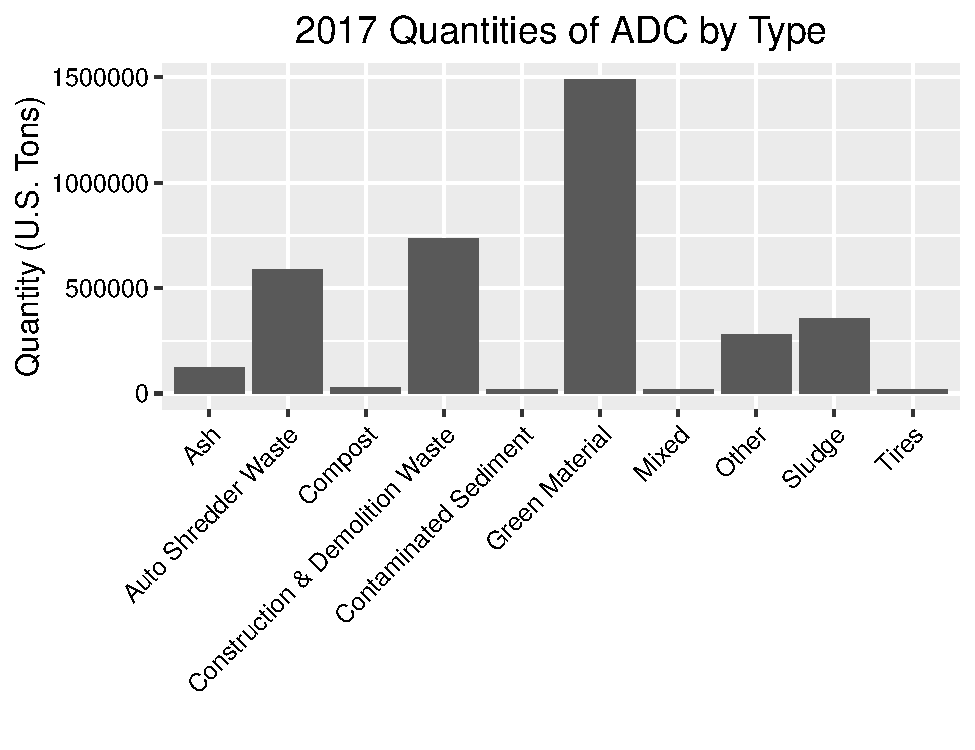
\includegraphics{SKo_Project_Template_files/figure-latex/explore_graphs2-1.pdf}
Figure 1: 2017 Quantities of ADC, separated by type

The geom\_bar function was used to create Figure 1. This figure shows
the 2017 ADC quantities per category. It is clear that waste categorized
as compost, contaminated sediment, mixed, and tires makes up a very
small part of the total ADC used.

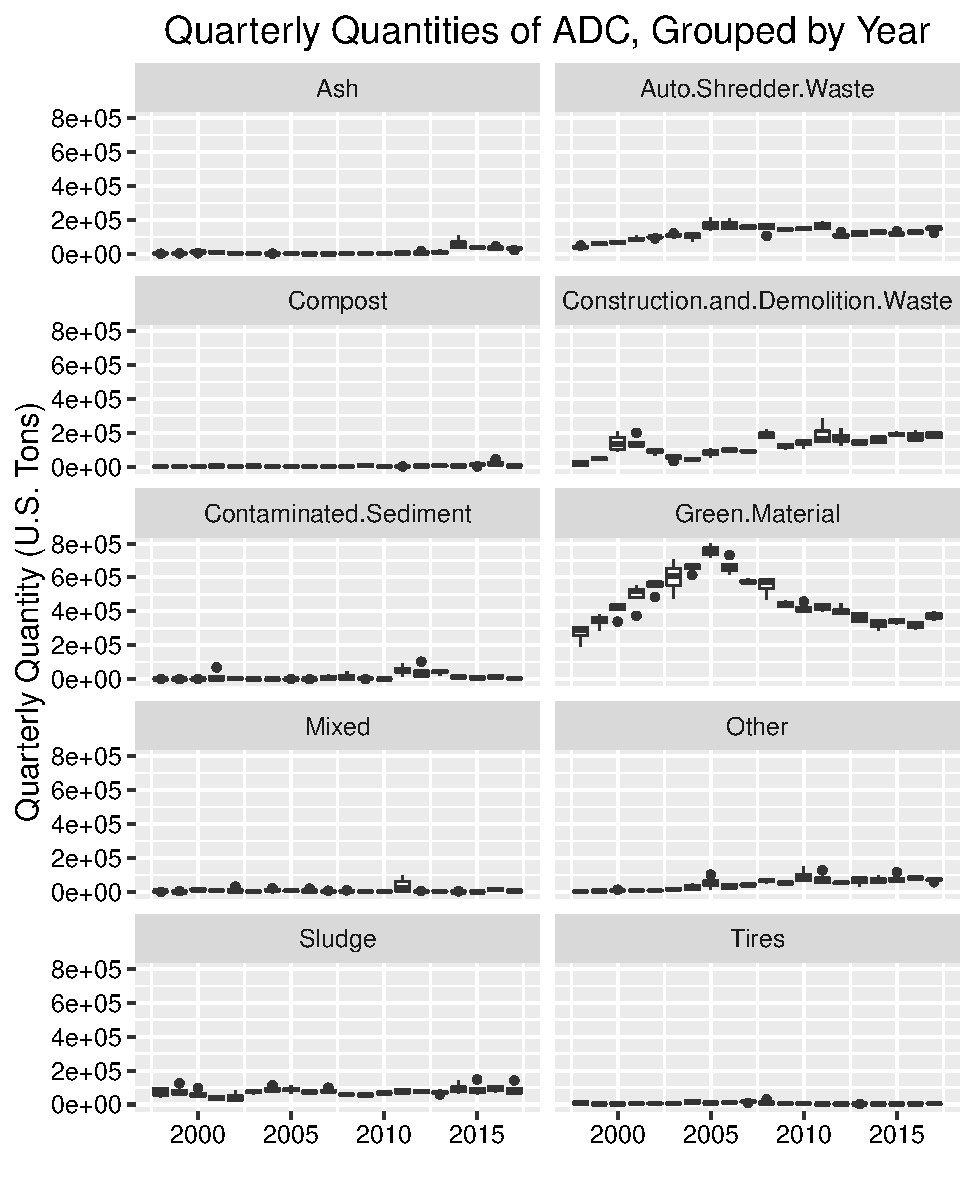
\includegraphics{SKo_Project_Template_files/figure-latex/explore_graphs3-1.pdf}
Figure 2: Quarterly quantities of ADC are grouped for each year. The
data is displayed by ADC type

The geom\_boxplot function was used to create Figure 2, which the
grouping function allowing the figure to display the data by year. The
plot was then faceted by ADC type to view the fluctuations of the
different ADC types over time. Auto shredder waste, and construction \&
demolition waste are seen to have experienced a gradual increase. The
box plots illustrate the spread of the quarterly data within each year.
Construction \& demolition waste, and green material are notable in that
they have a few years with very large spreads - C\&D had large spreads
in 2000 and 2010, and green material had large spreads from 1998-2005.

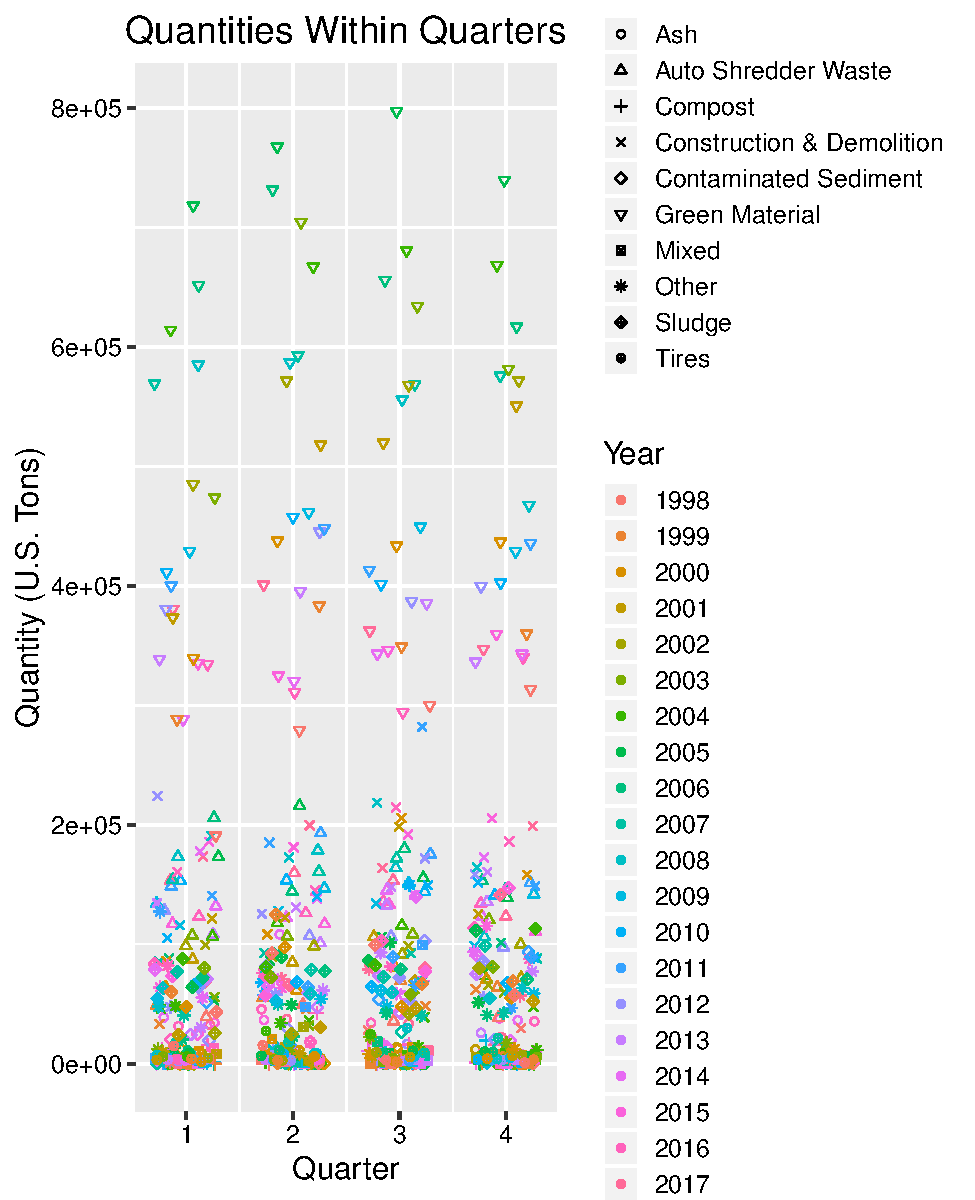
\includegraphics{SKo_Project_Template_files/figure-latex/explore_graphs4-1.pdf}
Figure 3: Quantities of ADC are grouped by the reporting quarter. The
report year is classified by color, and the ADC type is classified by
icon shape

gg\_plot was used to create Figure 3, which shows the quarterly
quantities of ADC split up by quarter. The jitter function was used to
prevent some overlap, allowing more of the points to be seen. The
characteristics of ADC type and year were illustrated the shape and
color of the point, respectively.

\newpage

\section{Analysis: Statistical Modeling \& Data
Visualization}\label{analysis-statistical-modeling-data-visualization}

\subsection{Test 1: Difference Between Report Quarters -
Analysis}\label{test-1-difference-between-report-quarters---analysis}

To assess trends in ADC corresponding to the yearly seasons, statistical
analysis was used to check for significant differences in total ADC
between report quarters 1, 2, 3, and 4. Since this analysis is on total
ADC, a new dataset was created that included data from years 1995-2017.
The quantity analyzed was the total (i.e.~the sum of all the types, per
year)

The test performed was a one-way ANOVA. The assumptions of a one-way
ANOVA are: 1) the observations are independent 2) the groups are
normally distributed 3) the variances among the groups are equal

Assumption 1 for independent observations cannot be checked from the
dataset, and was assumed to be true.

Assumption 2 for normal distribution was checked for each quarter using
the Shapiro Wilks test. The H0 for this test is that of normality, and
the p values for each of the groups was \textless{} 0.05 therefore these
groups were deemed not normally distributed.

A frequency polygon was used to view the distribution of each quarter,
which showed the data to be left skewed. A Q-Q plot was also used to
check normality, and found that the data does not match the 1:1 ratio
well. In an attempt to fix the departure from normality, a ln
transformation and an inverse transformation were used, but neither was
successful in making the data match a normal distribution.

Assumption 3 for homogeneity of variances was checked using the bartlett
test. The H0 for this test is that the variance is equal among the
groups. The p values were all \textgreater{} 0.05 therefore the
variances were deemed equal.

Since the data was deemed not normal, a Kruskal-Wallis, a non-parametric
test, was used instead of the one-way ANOVA. The Dunn test, a post-hoc
test, was also performed. The p values seen in the post-hoc test were
all much greater than 0.05, therefore the means of these groups were
found to not be significantly different from each other.

\begin{Shaded}
\begin{Highlighting}[]
\CommentTok{# create dataset with only total values, from 1995-2017}
\NormalTok{ADC_total_only <-}\StringTok{ }\NormalTok{ADC_raw }\OperatorTok
\StringTok{  }\KeywordTok{select}\NormalTok{(Report.Year, Report.Quarter, Total) }\CommentTok{# keep all columns except ADC Types}

\CommentTok{# convert column Report.Quarter into factor}
\KeywordTok{class}\NormalTok{(ADC_total_only}\OperatorTok{$}\NormalTok{Report.Quarter)}
\end{Highlighting}
\end{Shaded}

\begin{verbatim}
## [1] "integer"
\end{verbatim}

\begin{Shaded}
\begin{Highlighting}[]
\NormalTok{ADC_total_only}\OperatorTok{$}\NormalTok{Report.Quarter <-}\StringTok{ }\KeywordTok{as.factor}\NormalTok{(ADC_total_only}\OperatorTok{$}\NormalTok{Report.Quarter) }

\CommentTok{# save the dataset}
\KeywordTok{write.csv}\NormalTok{(ADC_total_only, }\DataTypeTok{row.names =} \OtherTok{FALSE}\NormalTok{, }
          \DataTypeTok{file =} \StringTok{"../Processed_Data/CalRecycle_ADC_totalsonly_processed.csv"}\NormalTok{)}

\CommentTok{# perform one-way ANOVA}
\CommentTok{# assumption #0: observations are independent }
\CommentTok{#(cannot be tested, but assumed to be independent)}

\CommentTok{# test assumption #1: normality}
\CommentTok{# null hypothesis is that the dataset is normally distributed}
\KeywordTok{shapiro.test}\NormalTok{(ADC_total_only}\OperatorTok{$}\NormalTok{Total[ADC_total_only}\OperatorTok{$}\NormalTok{Report.Quarter }\OperatorTok{==}\StringTok{ }\DecValTok{1}\NormalTok{]) }
\end{Highlighting}
\end{Shaded}

\begin{verbatim}
## 
##  Shapiro-Wilk normality test
## 
## data:  ADC_total_only$Total[ADC_total_only$Report.Quarter == 1]
## W = 0.90566, p-value = 0.03312
\end{verbatim}

\begin{Shaded}
\begin{Highlighting}[]
\CommentTok{# p-value = 0.03312}
\KeywordTok{shapiro.test}\NormalTok{(ADC_total_only}\OperatorTok{$}\NormalTok{Total[ADC_total_only}\OperatorTok{$}\NormalTok{Report.Quarter }\OperatorTok{==}\StringTok{ }\DecValTok{2}\NormalTok{]) }
\end{Highlighting}
\end{Shaded}

\begin{verbatim}
## 
##  Shapiro-Wilk normality test
## 
## data:  ADC_total_only$Total[ADC_total_only$Report.Quarter == 2]
## W = 0.89774, p-value = 0.02271
\end{verbatim}

\begin{Shaded}
\begin{Highlighting}[]
\CommentTok{# p-value = 0.02271}
\KeywordTok{shapiro.test}\NormalTok{(ADC_total_only}\OperatorTok{$}\NormalTok{Total[ADC_total_only}\OperatorTok{$}\NormalTok{Report.Quarter }\OperatorTok{==}\StringTok{ }\DecValTok{3}\NormalTok{]) }
\end{Highlighting}
\end{Shaded}

\begin{verbatim}
## 
##  Shapiro-Wilk normality test
## 
## data:  ADC_total_only$Total[ADC_total_only$Report.Quarter == 3]
## W = 0.87982, p-value = 0.00993
\end{verbatim}

\begin{Shaded}
\begin{Highlighting}[]
\CommentTok{# p-value = 0.00993}
\KeywordTok{shapiro.test}\NormalTok{(ADC_total_only}\OperatorTok{$}\NormalTok{Total[ADC_total_only}\OperatorTok{$}\NormalTok{Report.Quarter }\OperatorTok{==}\StringTok{ }\DecValTok{4}\NormalTok{]) }
\end{Highlighting}
\end{Shaded}

\begin{verbatim}
## 
##  Shapiro-Wilk normality test
## 
## data:  ADC_total_only$Total[ADC_total_only$Report.Quarter == 4]
## W = 0.83198, p-value = 0.001305
\end{verbatim}

\begin{Shaded}
\begin{Highlighting}[]
\CommentTok{# p-value = 0.001305}

\NormalTok{ADC_freq_poly <-}\StringTok{ }\KeywordTok{ggplot}\NormalTok{(ADC_total_only) }\OperatorTok{+}
\StringTok{  }\KeywordTok{geom_freqpoly}\NormalTok{(}\KeywordTok{aes}\NormalTok{(}\DataTypeTok{x =}\NormalTok{ Total, }\DataTypeTok{color =}\NormalTok{ Report.Quarter)) }\OperatorTok{+}\StringTok{ }
\StringTok{  }\KeywordTok{xlab}\NormalTok{(}\StringTok{"Quarterly Quantity (U.S. Tons)"}\NormalTok{) }\OperatorTok{+}\StringTok{ }
\StringTok{  }\KeywordTok{ylab}\NormalTok{(}\StringTok{"# of Records"}\NormalTok{) }\OperatorTok{+}\StringTok{ }
\StringTok{  }\KeywordTok{ggtitle}\NormalTok{(}\StringTok{"Frequency of Quarterly Quantities"}\NormalTok{)}
\KeywordTok{print}\NormalTok{(ADC_freq_poly) }\CommentTok{# appears to be left skewed}
\end{Highlighting}
\end{Shaded}

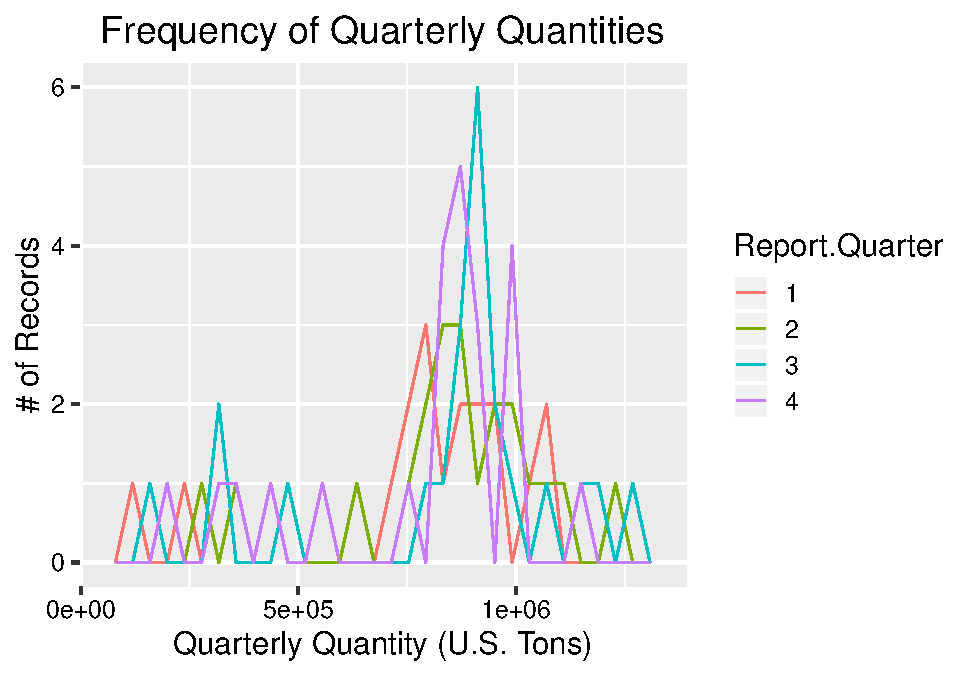
\includegraphics{SKo_Project_Template_files/figure-latex/Test1_1-1.pdf}

\begin{Shaded}
\begin{Highlighting}[]
\KeywordTok{qqnorm}\NormalTok{(ADC_total_only}\OperatorTok{$}\NormalTok{Total); }\KeywordTok{qqline}\NormalTok{(ADC_total_only}\OperatorTok{$}\NormalTok{Total) }
\end{Highlighting}
\end{Shaded}

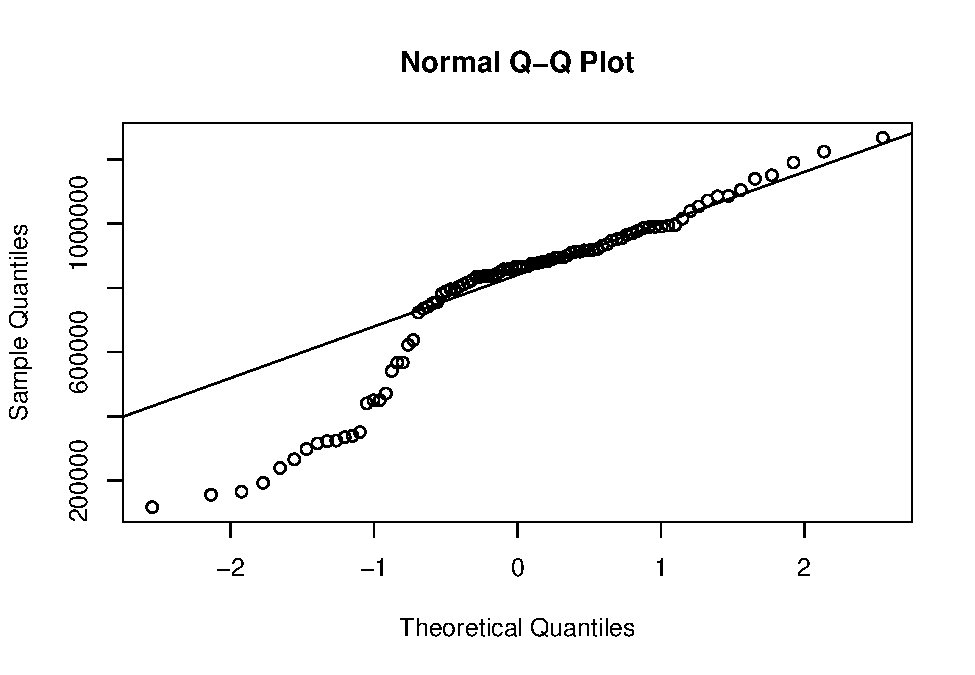
\includegraphics{SKo_Project_Template_files/figure-latex/Test1_1-2.pdf}

\begin{Shaded}
\begin{Highlighting}[]
\CommentTok{# does not match 1:1 ratio}

\CommentTok{# Try to fix departure from normality with ln of Total. }
\CommentTok{#Result is not improved, so keep non-transformed data}
\NormalTok{ADC_LogTotal <-}\StringTok{ }\KeywordTok{mutate}\NormalTok{(ADC_total_only, }\DataTypeTok{LogTotal =} \KeywordTok{log}\NormalTok{(Total))}
\KeywordTok{qqnorm}\NormalTok{(ADC_LogTotal}\OperatorTok{$}\NormalTok{LogTotal); }\KeywordTok{qqline}\NormalTok{(ADC_LogTotal}\OperatorTok{$}\NormalTok{LogTotal)}
\end{Highlighting}
\end{Shaded}

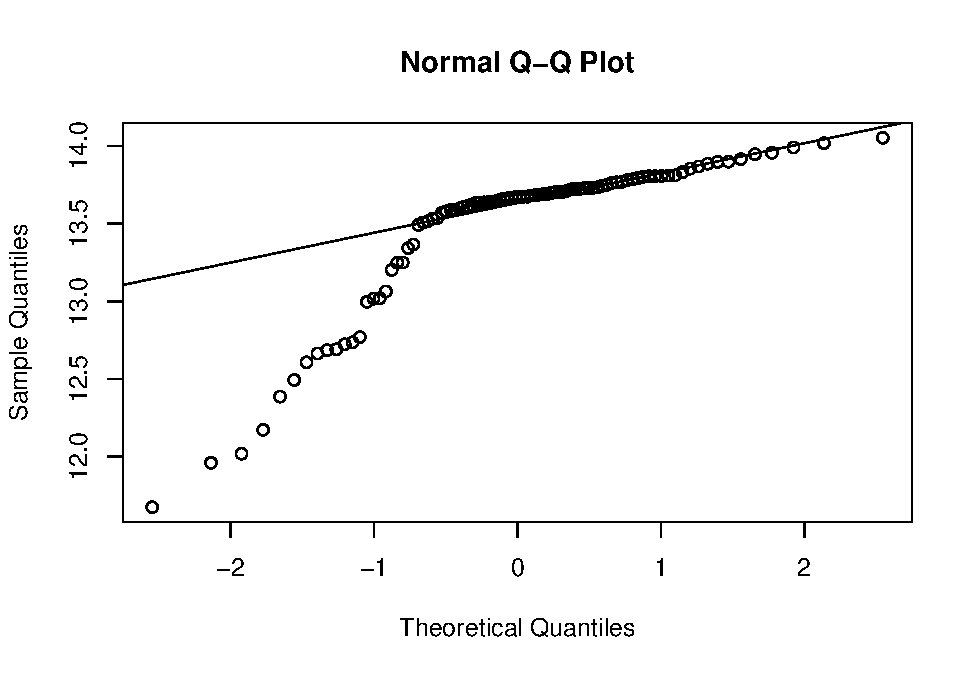
\includegraphics{SKo_Project_Template_files/figure-latex/Test1_1-3.pdf}

\begin{Shaded}
\begin{Highlighting}[]
\KeywordTok{bartlett.test}\NormalTok{(ADC_LogTotal}\OperatorTok{$}\NormalTok{LogTotal }\OperatorTok{~}\StringTok{ }\NormalTok{ADC_LogTotal}\OperatorTok{$}\NormalTok{Report.Quarter)}
\end{Highlighting}
\end{Shaded}

\begin{verbatim}
## 
##  Bartlett test of homogeneity of variances
## 
## data:  ADC_LogTotal$LogTotal by ADC_LogTotal$Report.Quarter
## Bartlett's K-squared = 1.1435, df = 3, p-value = 0.7666
\end{verbatim}

\begin{Shaded}
\begin{Highlighting}[]
\CommentTok{# Try to fix departure from normality with 1/Total. }
\CommentTok{#Result is not improved, so keep non-transformed data}
\NormalTok{ADC_InvTotal <-}\StringTok{ }\KeywordTok{mutate}\NormalTok{(ADC_total_only, }\DataTypeTok{InvTotal =} \DecValTok{1}\OperatorTok{/}\NormalTok{Total)}
\KeywordTok{qqnorm}\NormalTok{(ADC_InvTotal}\OperatorTok{$}\NormalTok{InvTotal); }\KeywordTok{qqline}\NormalTok{(ADC_InvTotal}\OperatorTok{$}\NormalTok{InvTotal)}
\end{Highlighting}
\end{Shaded}

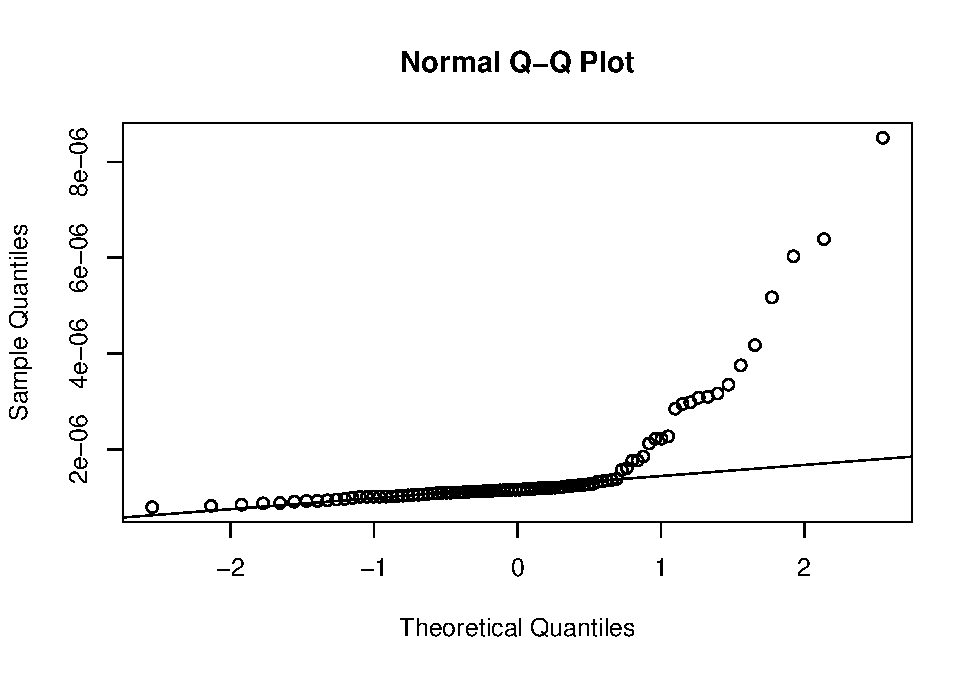
\includegraphics{SKo_Project_Template_files/figure-latex/Test1_1-4.pdf}

\begin{Shaded}
\begin{Highlighting}[]
\KeywordTok{bartlett.test}\NormalTok{(ADC_InvTotal}\OperatorTok{$}\NormalTok{InvTotal }\OperatorTok{~}\StringTok{ }\NormalTok{ADC_InvTotal}\OperatorTok{$}\NormalTok{Report.Quarter)}
\end{Highlighting}
\end{Shaded}

\begin{verbatim}
## 
##  Bartlett test of homogeneity of variances
## 
## data:  ADC_InvTotal$InvTotal by ADC_InvTotal$Report.Quarter
## Bartlett's K-squared = 6.519, df = 3, p-value = 0.08892
\end{verbatim}

\begin{Shaded}
\begin{Highlighting}[]
\CommentTok{# test assumption #2: equal variances among groups}

\CommentTok{# null hypothesis is that the variance is the same for the treatment groups}
\KeywordTok{bartlett.test}\NormalTok{(ADC_total_only}\OperatorTok{$}\NormalTok{Total }\OperatorTok{~}\StringTok{ }\NormalTok{ADC_total_only}\OperatorTok{$}\NormalTok{Report.Quarter) }
\end{Highlighting}
\end{Shaded}

\begin{verbatim}
## 
##  Bartlett test of homogeneity of variances
## 
## data:  ADC_total_only$Total by ADC_total_only$Report.Quarter
## Bartlett's K-squared = 0.44478, df = 3, p-value = 0.9308
\end{verbatim}

\begin{Shaded}
\begin{Highlighting}[]
\CommentTok{#p-value = 0.9308 # df = 3 (statistical power is very low)}

\CommentTok{# dataset is not normal, but does fulfill requirement for same variances.}
\CommentTok{#proceed with non-parametric tests.}

\CommentTok{# try non-parametric w/ post hoc, bc sample size is on the smaller end for parametric}
\NormalTok{ADC_quarter_kw <-}\StringTok{ }\KeywordTok{kruskal.test}\NormalTok{(ADC_total_only}\OperatorTok{$}\NormalTok{Total }\OperatorTok{~}\StringTok{ }\NormalTok{ADC_total_only}\OperatorTok{$}\NormalTok{Report.Quarter)}
\NormalTok{ADC_quarter_kw}
\end{Highlighting}
\end{Shaded}

\begin{verbatim}
## 
##  Kruskal-Wallis rank sum test
## 
## data:  ADC_total_only$Total by ADC_total_only$Report.Quarter
## Kruskal-Wallis chi-squared = 3.4581, df = 3, p-value = 0.3262
\end{verbatim}

\begin{Shaded}
\begin{Highlighting}[]
\KeywordTok{dunnTest}\NormalTok{(ADC_total_only}\OperatorTok{$}\NormalTok{Total, ADC_total_only}\OperatorTok{$}\NormalTok{Report.Quarter)}
\end{Highlighting}
\end{Shaded}

\begin{verbatim}
##   Comparison           Z    P.unadj     P.adj
## 1      1 - 2 -1.08778370 0.27669061 1.0000000
## 2      1 - 3 -1.84978446 0.06434462 0.3860677
## 3      2 - 3 -0.76200076 0.44605955 0.8921191
## 4      1 - 4 -1.00495753 0.31491730 1.0000000
## 5      2 - 4  0.08282617 0.93398976 0.9339898
## 6      3 - 4  0.84482693 0.39820748 1.0000000
\end{verbatim}

\subsubsection{Test 1: Result}\label{test-1-result}

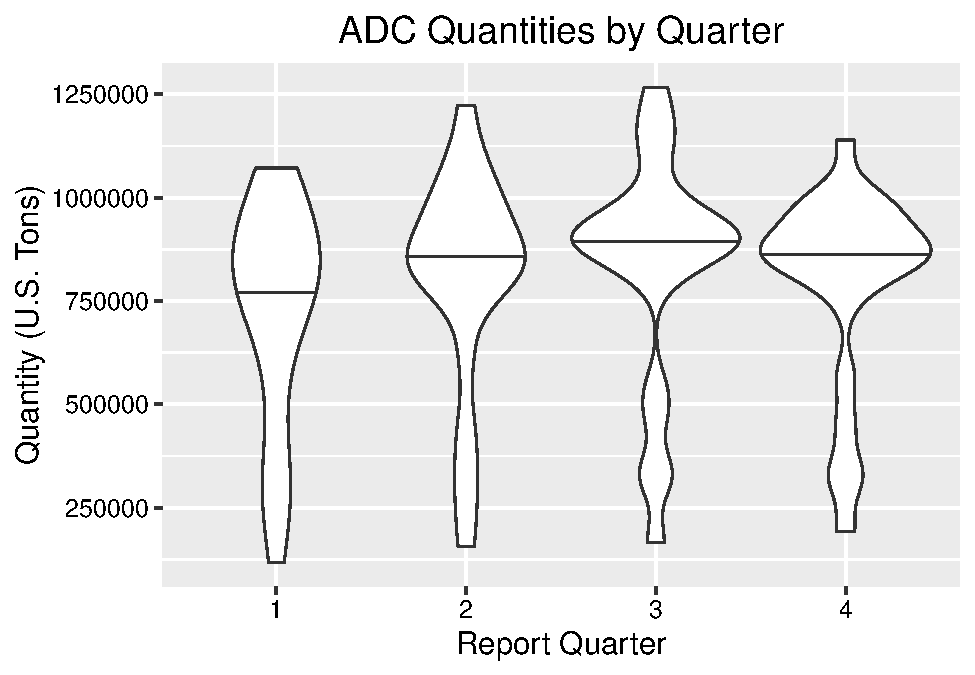
\includegraphics{SKo_Project_Template_files/figure-latex/Test1_2-1.pdf}
Figure 4: Quantities of ADC are grouped by quarter. The height of the
bar described the spread of the data, a the width of the bar describes
the number of records at each quantity

Figure 4 illustrates the numerical findings of the dunn test - that the
means of the quarters are not significantly different from one another.
The means of these groups is illustrated by the black horizonal lines,
which visually appear to be at similar quantities.

\subsection{Test 2: Linear Model -
Analysis}\label{test-2-linear-model---analysis}

The next test is to create a linear model of the quarterly values over
time, and plot the model over the data points to visualize the fit. If
the model is a good fit, the equation could be used to predict future
quantities of ADC. Since this model does not evaluate the ADC quantities
split up by type, the analysis is on the data from years 1995-2017. The
quantity analyzed was the total (i.e.~the sum of all the types, per
quarter). To prepare this data for analysis, the quarter+year
combinations were transformed into dates. The following dates were used
for each quarter: Q1: Mar 31 Q2: Jun 30 Q3: Sep 30 Q4: Dec 31 These
dates represent the end of each report quarter.

The assumptions for using a linear model are the same as that of the
one-way ANOVA: 1) the observations are independent 2) the groups are
normally distributed 3) the variances among the groups are equal

These were checked in Test 1. The data was not seen to be normal, but
the group variances were found homogenous, so a lm is attempted.

The model uses 1 dependent variable = quarterly quantity, and 1
independent variable = time. The equation was found to be as follows:
Quarterly quantity = 73.14*Date - 190264.58. This signifies that for a 1
unit increase in the date, the model predicts there to be a 73.14 ton
increase in the ADC quantity.

The adjusted R-squared value was seen to be 0.4433, which means that the
model explains 44.33\% of the variation. The p-value was found to be
2.694e-13.

\begin{Shaded}
\begin{Highlighting}[]
\CommentTok{# assumptions for lm (independent observation, normal distribution, }
\CommentTok{#equal variances among groups) checked in Test 1. data is not normal, }
\CommentTok{#but group variances are equal. proceed with lm}

\CommentTok{# create dates corresponding to year & quarter combination}
\CommentTok{# Q1: Mar 31}
\CommentTok{# Q2: Jun 30}
\CommentTok{# Q3: Sep 30}
\CommentTok{# Q4: Dec 31}

\CommentTok{# create dataframe of month-date}
\NormalTok{quarters_to_dates <-}\StringTok{ }\KeywordTok{data.frame}\NormalTok{(}\StringTok{"Quarter"}\NormalTok{ =}\StringTok{ }\KeywordTok{as.factor}\NormalTok{(}\DecValTok{1}\OperatorTok{:}\DecValTok{4}\NormalTok{), }
          \StringTok{"Month.Date"}\NormalTok{ =}\StringTok{ }\KeywordTok{c}\NormalTok{(}\StringTok{'3-31'}\NormalTok{, }\StringTok{'6-30'}\NormalTok{, }\StringTok{'9-30'}\NormalTok{, }\StringTok{'12-31'}\NormalTok{))}

\CommentTok{# create new dataframe with dates}
\NormalTok{ADC_fulldate <-}\StringTok{ }\NormalTok{ADC_total_only }\OperatorTok\StringTok{ }
\StringTok{  }\KeywordTok{inner_join}\NormalTok{(quarters_to_dates, }\DataTypeTok{by =} \KeywordTok{c}\NormalTok{(}\StringTok{"Report.Quarter"}\NormalTok{ =}\StringTok{  "Quarter"}\NormalTok{)) }\OperatorTok
\StringTok{  }\KeywordTok{unite}\NormalTok{(}\StringTok{'Quarter.End.Date'}\NormalTok{, }\KeywordTok{c}\NormalTok{(Report.Year, Month.Date), }\DataTypeTok{sep =} \StringTok{"-"}\NormalTok{, }\DataTypeTok{remove =} \OtherTok{FALSE}\NormalTok{)}

\NormalTok{ADC_fulldate}\OperatorTok{$}\NormalTok{Quarter.End.Date <-}\StringTok{ }\KeywordTok{as.Date}\NormalTok{(ADC_fulldate}\OperatorTok{$}\NormalTok{Quarter.End.Date, }\StringTok{"%Y-%m-%d"}\NormalTok{)}
\KeywordTok{class}\NormalTok{(ADC_fulldate}\OperatorTok{$}\NormalTok{Quarter.End.Date)}
\end{Highlighting}
\end{Shaded}

\begin{verbatim}
## [1] "Date"
\end{verbatim}

\begin{Shaded}
\begin{Highlighting}[]
\CommentTok{# create initial plot to visualize the data}
\KeywordTok{ggplot}\NormalTok{(ADC_fulldate, }\KeywordTok{aes}\NormalTok{(}\DataTypeTok{x =}\NormalTok{ Quarter.End.Date, }\DataTypeTok{y =}\NormalTok{ Total)) }\OperatorTok{+}
\StringTok{  }\KeywordTok{geom_point}\NormalTok{() }\OperatorTok{+}\StringTok{ }
\StringTok{  }\KeywordTok{xlab}\NormalTok{(}\StringTok{""}\NormalTok{) }\OperatorTok{+}\StringTok{ }
\StringTok{  }\KeywordTok{ylab}\NormalTok{(}\StringTok{"ADC Quantity (U.S. Tons)"}\NormalTok{) }\OperatorTok{+}
\StringTok{  }\KeywordTok{ggtitle}\NormalTok{(}\StringTok{"Quarterly Quantities of ADC"}\NormalTok{)}
\end{Highlighting}
\end{Shaded}

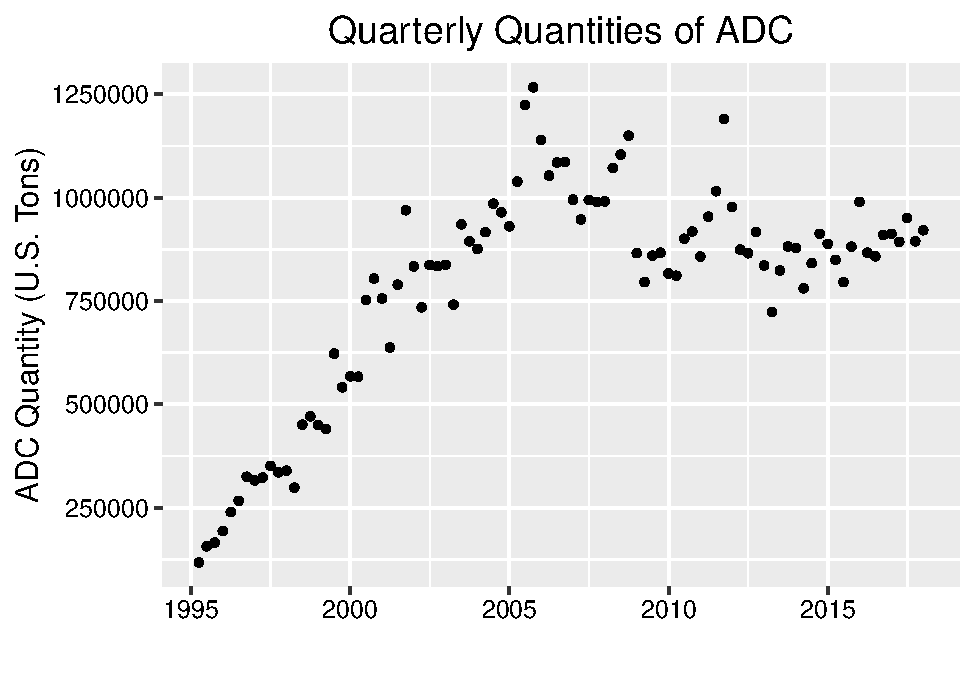
\includegraphics{SKo_Project_Template_files/figure-latex/Test2_1-1.pdf}

\begin{Shaded}
\begin{Highlighting}[]
\CommentTok{# create lm}
\NormalTok{ADC_date_lm <-}\StringTok{ }\KeywordTok{lm}\NormalTok{(}\DataTypeTok{data =}\NormalTok{ ADC_fulldate, Total }\OperatorTok{~}\StringTok{ }\NormalTok{Quarter.End.Date)}
\NormalTok{ADC_date_lm }\CommentTok{# Total = 73.14*Quarter.End.Date - 190264.58}
\end{Highlighting}
\end{Shaded}

\begin{verbatim}
## 
## Call:
## lm(formula = Total ~ Quarter.End.Date, data = ADC_fulldate)
## 
## Coefficients:
##      (Intercept)  Quarter.End.Date  
##       -190264.58             73.14
\end{verbatim}

\begin{Shaded}
\begin{Highlighting}[]
\KeywordTok{summary}\NormalTok{(ADC_date_lm) }
\end{Highlighting}
\end{Shaded}

\begin{verbatim}
## 
## Call:
## lm(formula = Total ~ Quarter.End.Date, data = ADC_fulldate)
## 
## Residuals:
##     Min      1Q  Median      3Q     Max 
## -366483 -153515  -45160  167108  502499 
## 
## Coefficients:
##                    Estimate Std. Error t value Pr(>|t|)    
## (Intercept)      -1.903e+05  1.160e+05   -1.64    0.104    
## Quarter.End.Date  7.314e+01  8.534e+00    8.57 2.69e-13 ***
## ---
## Signif. codes:  0 '***' 0.001 '**' 0.01 '*' 0.05 '.' 0.1 ' ' 1
## 
## Residual standard error: 198500 on 90 degrees of freedom
## Multiple R-squared:  0.4494, Adjusted R-squared:  0.4433 
## F-statistic: 73.45 on 1 and 90 DF,  p-value: 2.694e-13
\end{verbatim}

\begin{Shaded}
\begin{Highlighting}[]
\CommentTok{# Adjusted R-squared:  0.4433 (date explains 44.33% of variation in total),}
\CommentTok{#p-value: 2.694e-13}

\CommentTok{# check normality of residuals}
\KeywordTok{par}\NormalTok{(}\DataTypeTok{mfrow=}\KeywordTok{c}\NormalTok{(}\DecValTok{2}\NormalTok{,}\DecValTok{2}\NormalTok{))}
\KeywordTok{plot}\NormalTok{(ADC_date_lm) }\CommentTok{# QQ of residuals looks relatively normal}
\end{Highlighting}
\end{Shaded}

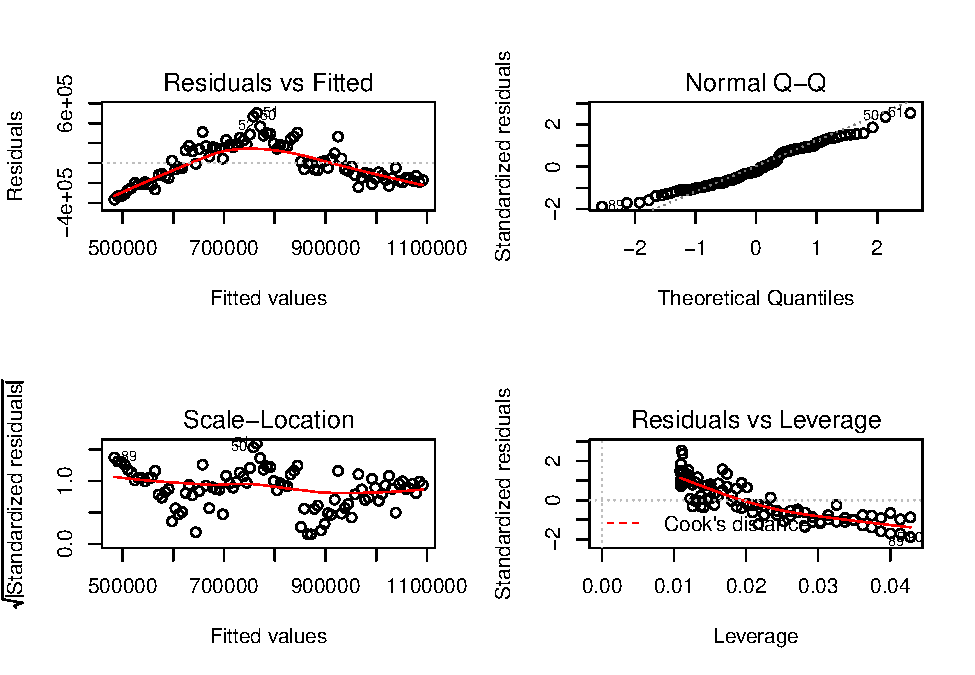
\includegraphics{SKo_Project_Template_files/figure-latex/Test2_1-2.pdf}

\subsubsection{Test 2: Result}\label{test-2-result}

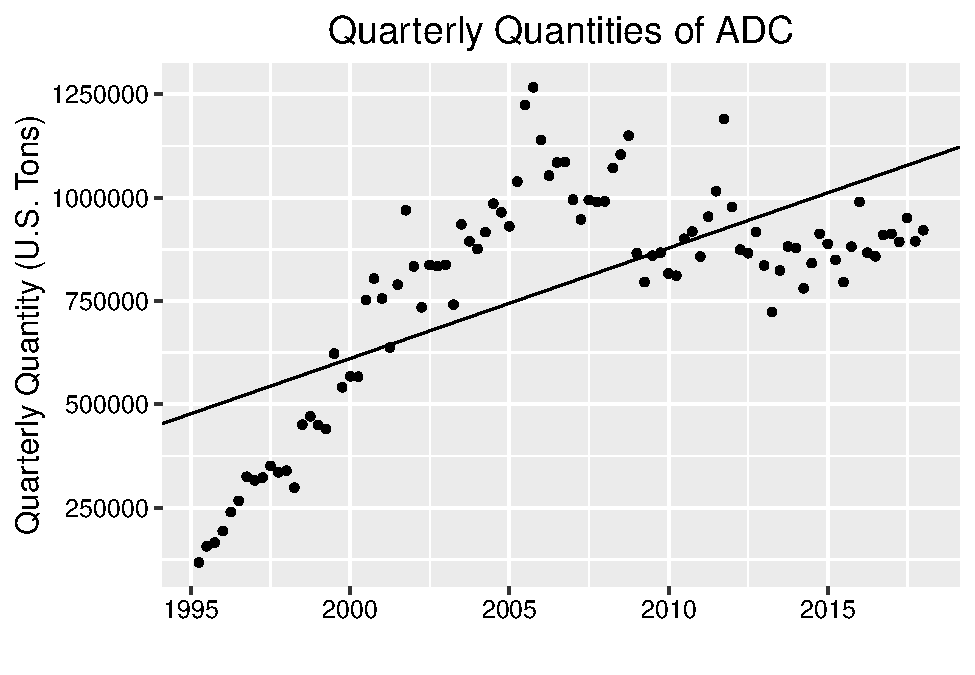
\includegraphics{SKo_Project_Template_files/figure-latex/Test2_2-1.pdf}
Figure 5: Quarterly quantities of ADC are plotted by time, and fit with
the equation y = 73.14*time -190264.58

Figure 5 shows the individual data points plotted over time, overlaid
with the model represented by the line. The model does follow the same
upward trend that the points show, but visually the model does not
appear to be a good fit for the data. The points show a peak around 2006
and level off after that, which is not represented in the model.

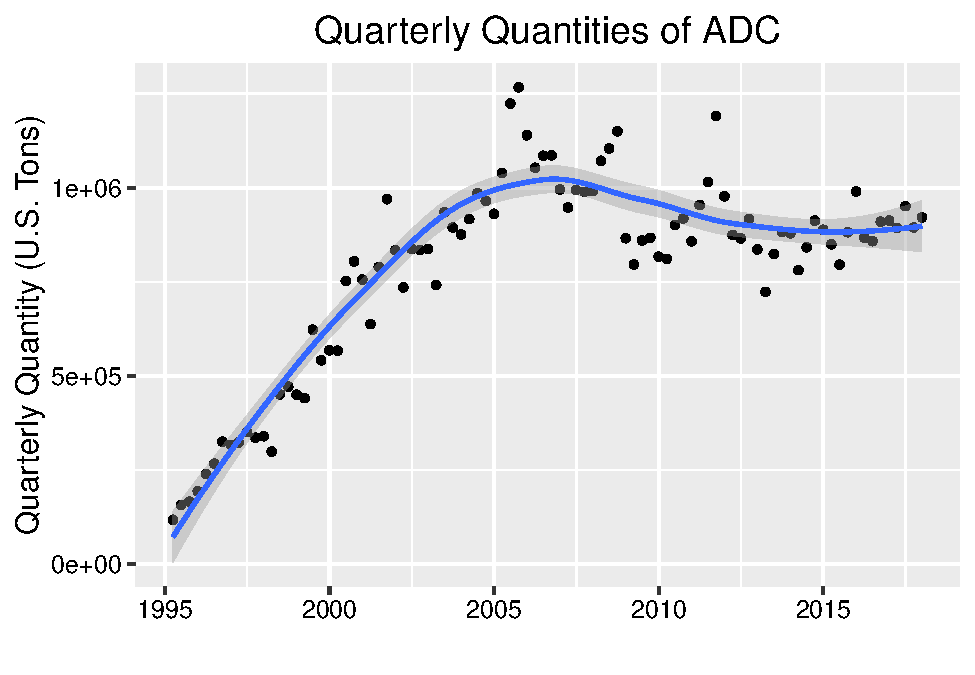
\includegraphics{SKo_Project_Template_files/figure-latex/Test2_3-1.pdf}
Figure 6: Quarterly quantities of ADC are plotted by time, and fit with
a Loess Regression

Figure 6 shows the individual data points plotted over time, overlaid
with a Loess regression. The Loess regression appears to be a much
better fit to the data points visually. The model is represented by the
blue line and the confidence interval of the model is represented by the
gray area surrounding the line.

\subsection{Test 3: Changepoint in Construction \& Demolition -
Analysis}\label{test-3-changepoint-in-construction-demolition---analysis}

Test 3 assessed construction \& demolition ADC quantities over time,
checking for changepoints in the data. Since this analysis is on
type-specific ADC, only data from years 1998-2017 was used. The data was
limited to only C\&D waste by using the select function.

The determine the type of test that should be used, the following 2
assumptions were evaluated: 1) the observations are independent 2) the
groups are normally distributed

Assumption 1 for independent observations cannot be checked from the
dataset, and was assumed to be true.

Assumption 2 for normal distribution was checked using the Shapiro Wilks
test. The H0 for this test is that of normality, and the p value = 0.4,
therefore this data set was deemed to be normally distributed.

A histogram was used to view the distribution, which appears visually to
have a normal distribution. A Q-Q plot was also used to check normality,
and found that the data matches the 1:1 ratio well.

Although the data was found to be normal, the non-parametric Pettitt
test was used to determine a shift in the central tendancy of the time
series, because the sample size is not very large. The Pettitt test
found p = 3.2e-10, which is \textless{} 0.05. The change point was
identified at time `40', which corresponds to a time between Q4 2007 \&
Q1 2008 = \textasciitilde{} 2008-02-14.

A separate Mann-Kendall was run for each section (before and after the
change point). In the block of points after time `40', the corresponding
p = 0.01308, which indicates that there is likely a second change point
in that block. A Pettitt test was run on that chunk and found a second
change point corresponding to a time between Q4 2014 \& Q1 2015 =
\textasciitilde{} 2015-02-14.

\begin{Shaded}
\begin{Highlighting}[]
\CommentTok{# create dataframe with dates}
\NormalTok{quarters_to_dates}\OperatorTok{$}\NormalTok{Quarter <-}\StringTok{ }\KeywordTok{as.integer}\NormalTok{(quarters_to_dates}\OperatorTok{$}\NormalTok{Quarter)}

\NormalTok{CD_only <-}\StringTok{ }\NormalTok{ADC_data }\OperatorTok\StringTok{ }
\StringTok{  }\KeywordTok{select}\NormalTok{(Report.Year, Report.Quarter, Construction.and.Demolition.Waste) }\OperatorTok
\StringTok{  }\KeywordTok{inner_join}\NormalTok{(quarters_to_dates, }\DataTypeTok{by =} \KeywordTok{c}\NormalTok{(}\StringTok{"Report.Quarter"}\NormalTok{ =}\StringTok{  "Quarter"}\NormalTok{)) }\OperatorTok
\StringTok{  }\KeywordTok{unite}\NormalTok{(}\StringTok{'Quarter.End.Date'}\NormalTok{, }\KeywordTok{c}\NormalTok{(Report.Year, Month.Date), }\DataTypeTok{sep =} \StringTok{"-"}\NormalTok{) }\OperatorTok
\StringTok{  }\KeywordTok{select}\NormalTok{(}\OperatorTok{-}\NormalTok{Report.Quarter)}

\NormalTok{CD_only}\OperatorTok{$}\NormalTok{Quarter.End.Date <-}\StringTok{ }\KeywordTok{as.Date}\NormalTok{(CD_only}\OperatorTok{$}\NormalTok{Quarter.End.Date, }\StringTok{'%Y-%m-%d'}\NormalTok{) }
\CommentTok{# format column as date}

\CommentTok{# arrange data from oldest to newest}
\NormalTok{CD_only <-}\StringTok{ }\NormalTok{CD_only }\OperatorTok\StringTok{ }
\StringTok{  }\KeywordTok{arrange}\NormalTok{(Quarter.End.Date)}

\CommentTok{# create initial plot to visualize the data}
\KeywordTok{ggplot}\NormalTok{(CD_only, }\KeywordTok{aes}\NormalTok{(}\DataTypeTok{x =}\NormalTok{ Quarter.End.Date, }\DataTypeTok{y =}\NormalTok{ Construction.and.Demolition.Waste)) }\OperatorTok{+}
\StringTok{  }\KeywordTok{geom_point}\NormalTok{() }\OperatorTok{+}\StringTok{ }
\StringTok{  }\KeywordTok{xlab}\NormalTok{(}\StringTok{""}\NormalTok{) }\OperatorTok{+}\StringTok{ }
\StringTok{  }\KeywordTok{ylab}\NormalTok{(}\StringTok{"C&D Quantity (U.S. Tons)"}\NormalTok{) }\OperatorTok{+}\StringTok{ }
\StringTok{  }\KeywordTok{ggtitle}\NormalTok{(}\StringTok{"Construction & Demolition Quarterly Quantities"}\NormalTok{)}
\end{Highlighting}
\end{Shaded}

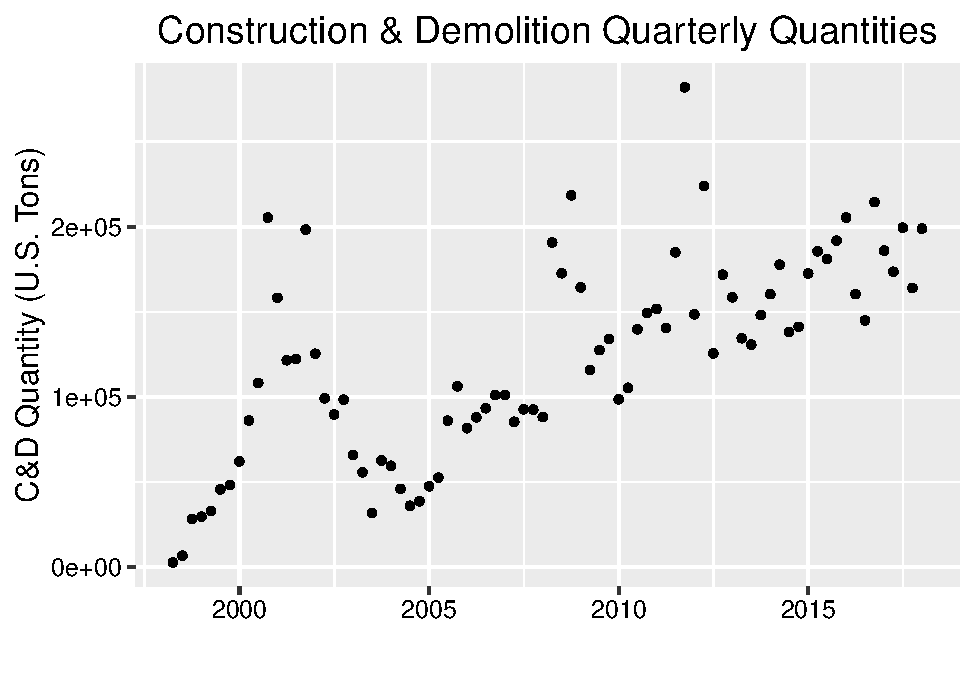
\includegraphics{SKo_Project_Template_files/figure-latex/Test3_1-1.pdf}

\begin{Shaded}
\begin{Highlighting}[]
\CommentTok{# check normality for C&D waste specifically}
\KeywordTok{shapiro.test}\NormalTok{(CD_only}\OperatorTok{$}\NormalTok{Construction.and.Demolition.Waste) }
\end{Highlighting}
\end{Shaded}

\begin{verbatim}
## 
##  Shapiro-Wilk normality test
## 
## data:  CD_only$Construction.and.Demolition.Waste
## W = 0.9837, p-value = 0.4028
\end{verbatim}

\begin{Shaded}
\begin{Highlighting}[]
\CommentTok{# p-value = 0.4028, inferring that the data is normal}

\KeywordTok{ggplot}\NormalTok{(CD_only) }\OperatorTok{+}
\StringTok{  }\KeywordTok{geom_histogram}\NormalTok{(}\KeywordTok{aes}\NormalTok{(}\DataTypeTok{x =}\NormalTok{ Construction.and.Demolition.Waste)) }\OperatorTok{+}\StringTok{ }
\StringTok{  }\KeywordTok{xlab}\NormalTok{(}\StringTok{"Quarterly C&D (U.S. Tons)"}\NormalTok{) }\OperatorTok{+}
\StringTok{  }\KeywordTok{ylab}\NormalTok{(}\StringTok{"Count"}\NormalTok{) }\OperatorTok{+}\StringTok{ }
\StringTok{  }\KeywordTok{ggtitle}\NormalTok{(}\StringTok{"Count of Quarterly C&D Quantities"}\NormalTok{)}
\end{Highlighting}
\end{Shaded}

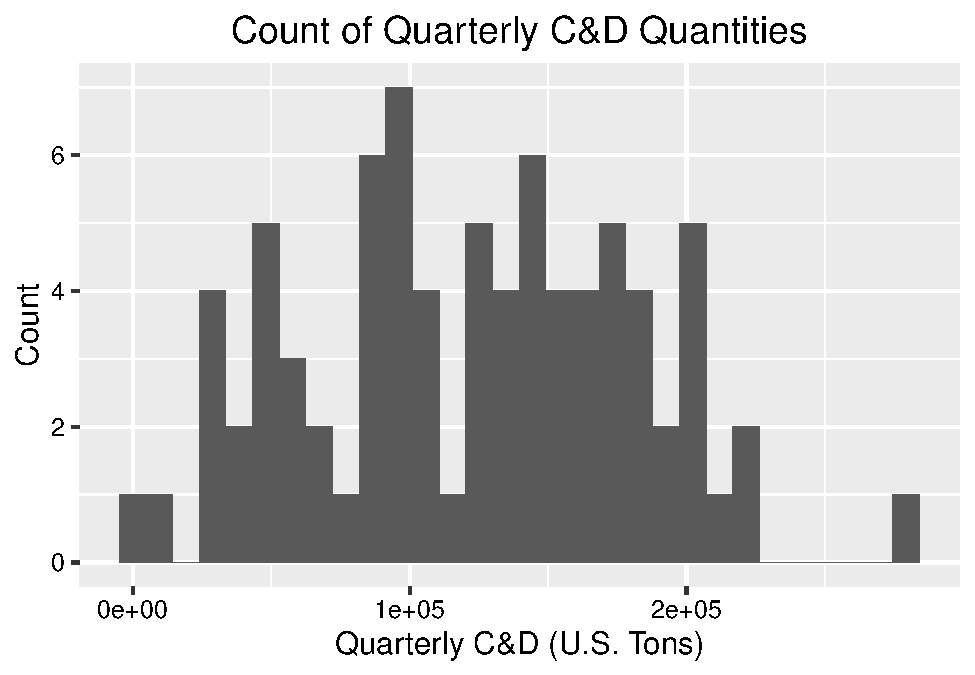
\includegraphics{SKo_Project_Template_files/figure-latex/Test3_1-2.pdf}

\begin{Shaded}
\begin{Highlighting}[]
\KeywordTok{qqnorm}\NormalTok{(CD_only}\OperatorTok{$}\NormalTok{Construction.and.Demolition.Waste);}
\KeywordTok{qqline}\NormalTok{(CD_only}\OperatorTok{$}\NormalTok{Construction.and.Demolition.Waste) }\CommentTok{# matches 1:1 ratio pretty well}
\end{Highlighting}
\end{Shaded}

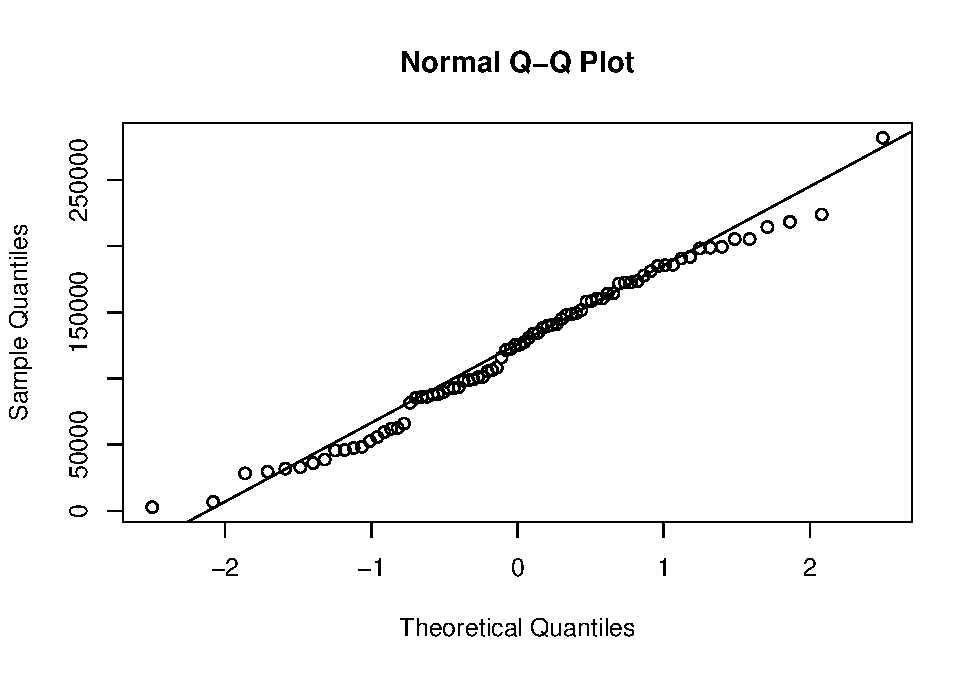
\includegraphics{SKo_Project_Template_files/figure-latex/Test3_1-3.pdf}

\begin{Shaded}
\begin{Highlighting}[]
\CommentTok{# use Pettitt's test (nonparametric) to determine whether there is a shift }
\CommentTok{#in the central tendency of the time series. }
\KeywordTok{pettitt.test}\NormalTok{(CD_only}\OperatorTok{$}\NormalTok{Construction.and.Demolition.Waste) }\CommentTok{# change point at time 40}
\end{Highlighting}
\end{Shaded}

\begin{verbatim}
## 
##  Pettitt's test for single change-point detection
## 
## data:  CD_only$Construction.and.Demolition.Waste
## U* = 1396, p-value = 3.2e-10
## alternative hypothesis: two.sided
## sample estimates:
## probable change point at time K 
##                              40
\end{verbatim}

\begin{Shaded}
\begin{Highlighting}[]
\CommentTok{# Run separate Mann-Kendall for each section}
\KeywordTok{mk.test}\NormalTok{(CD_only}\OperatorTok{$}\NormalTok{Construction.and.Demolition.Waste[}\DecValTok{1}\OperatorTok{:}\DecValTok{40}\NormalTok{])}
\end{Highlighting}
\end{Shaded}

\begin{verbatim}
## 
##  Mann-Kendall trend test
## 
## data:  CD_only$Construction.and.Demolition.Waste[1:40]
## z = 1.736, n = 40, p-value = 0.08256
## alternative hypothesis: true S is not equal to 0
## sample estimates:
##            S         varS          tau 
##  150.0000000 7366.6666667    0.1923077
\end{verbatim}

\begin{Shaded}
\begin{Highlighting}[]
\KeywordTok{mk.test}\NormalTok{(CD_only}\OperatorTok{$}\NormalTok{Construction.and.Demolition.Waste[}\DecValTok{41}\OperatorTok{:}\DecValTok{80}\NormalTok{])}
\end{Highlighting}
\end{Shaded}

\begin{verbatim}
## 
##  Mann-Kendall trend test
## 
## data:  CD_only$Construction.and.Demolition.Waste[41:80]
## z = 2.4817, n = 40, p-value = 0.01308
## alternative hypothesis: true S is not equal to 0
## sample estimates:
##           S        varS         tau 
##  214.000000 7366.666667    0.274359
\end{verbatim}

\begin{Shaded}
\begin{Highlighting}[]
\CommentTok{# Is there a second change point?}
\KeywordTok{pettitt.test}\NormalTok{(CD_only}\OperatorTok{$}\NormalTok{Construction.and.Demolition.Waste[}\DecValTok{41}\OperatorTok{:}\DecValTok{80}\NormalTok{])}
\end{Highlighting}
\end{Shaded}

\begin{verbatim}
## 
##  Pettitt's test for single change-point detection
## 
## data:  CD_only$Construction.and.Demolition.Waste[41:80]
## U* = 203, p-value = 0.04614
## alternative hypothesis: two.sided
## sample estimates:
## probable change point at time K 
##                              27
\end{verbatim}

\begin{Shaded}
\begin{Highlighting}[]
\CommentTok{# position 27, so 41+27 = change point at time 68}

\CommentTok{# Run separate Mann-Kendall for new section}
\KeywordTok{mk.test}\NormalTok{(CD_only}\OperatorTok{$}\NormalTok{Construction.and.Demolition.Waste[}\DecValTok{69}\OperatorTok{:}\DecValTok{80}\NormalTok{]) }
\end{Highlighting}
\end{Shaded}

\begin{verbatim}
## 
##  Mann-Kendall trend test
## 
## data:  CD_only$Construction.and.Demolition.Waste[69:80]
## z = 0.068573, n = 12, p-value = 0.9453
## alternative hypothesis: true S is not equal to 0
## sample estimates:
##            S         varS          tau 
##   2.00000000 212.66666667   0.03030303
\end{verbatim}

\begin{Shaded}
\begin{Highlighting}[]
\CommentTok{# p-value = 0.9453, not likely a 3rd change point}

\CommentTok{# Is there a third change point?}
\KeywordTok{pettitt.test}\NormalTok{(CD_only}\OperatorTok{$}\NormalTok{Construction.and.Demolition.Waste[}\DecValTok{69}\OperatorTok{:}\DecValTok{80}\NormalTok{]) }
\end{Highlighting}
\end{Shaded}

\begin{verbatim}
## 
##  Pettitt's test for single change-point detection
## 
## data:  CD_only$Construction.and.Demolition.Waste[69:80]
## U* = 12, p-value = 1.261
## alternative hypothesis: two.sided
## sample estimates:
## probable change point at time K 
##                               6
\end{verbatim}

\begin{Shaded}
\begin{Highlighting}[]
\CommentTok{# p-value = p-value = 1.261, no 3rd change point}

\CommentTok{# years corresponding to changepoints}
\NormalTok{changepoint1 <-}\StringTok{ }\NormalTok{CD_only}\OperatorTok{$}\NormalTok{Quarter.End.Date[}\DecValTok{40}\NormalTok{] }
\CommentTok{# between Q4 2007 & Q1 2008 = ~ 2008-02-14}
\NormalTok{changepoint2 <-}\StringTok{ }\NormalTok{CD_only}\OperatorTok{$}\NormalTok{Quarter.End.Date[}\DecValTok{68}\NormalTok{] }
\CommentTok{# between Q4 2014 & Q1 2015 = ~ 2015-02-14}
\end{Highlighting}
\end{Shaded}

\subsubsection{Test 3: Result}\label{test-3-result}

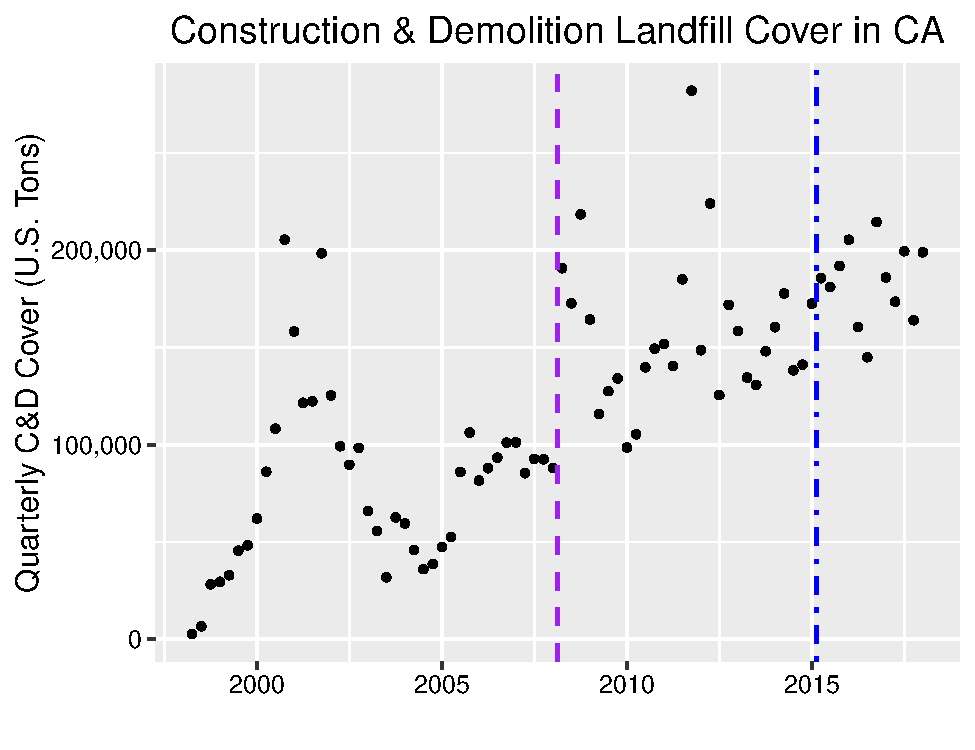
\includegraphics{SKo_Project_Template_files/figure-latex/Test3_2-1.pdf}
Figure 7: Quarterly quantities of Construction \& Demolition ADC are
plotted by time, and the 2 changepoints are marked with dotted lines

Figure 7 shows the quarterly C\&D quantities plotted over time, with
changepoints highlighted at \textasciitilde{} 2008-02-14 (in purple) and
\textasciitilde{} 2015-02-14 (blue). There appears to be a changepoint
at around 2002, but the statistical test did not detect a changepoint
there. It is possible that is due to the sample size. Also, the
changepoint detected at \textasciitilde{} 2015-02-14 (blue) does not
seem to be represented by the data points. This may also be due to the
small sample size, or could be influenced by the high quantity values
seen around 2012.

\newpage

\section{Summary and Conclusions}\label{summary-and-conclusions}

The analysis of the quantity of ADC used in each reporting quarter found
that the means of the quarters are not significantly different from one
another. This was found quantitatively via the dunn post-hoc test, but
can also be seen visually from a violin plot. This lack of a quarterly
trend infers that the supply of ADC (or of earthen material) is
relatively constant across the year. This could be a nationwide trend,
or a special effect from California's temperate climate allowing for
relatively similar weather (and thus growing season) year-round.

When attempting to model quarterly ADC quantities as a function of time
the linear model was a moderate fit, explaining \textasciitilde{}44\% of
the variation. Visually though, the model equation (Quarterly Quantity =
73.14*Date - 190264.58) did not appear to be a good fit for the data
points. The Loess regression was seen to provide a much better fit
visually. For future studies, models beyond the y-mx+b equation would
likely be better predictors of quantity of ADC over time.

For construction \& demolition ADC specifically, there were 2
changepoints in the quantities over time - one around 2008-02-14, and
another around 2015-02-14. Literature research did not show an
association of either of these dates with a major change in regulation
surrounding landfill diversion standards, but there may be other policy
factors influencing these findings. The trends in C\&D waste would be
useful information to share with landfill operators to help them predict
influxes in the production of hydrogen sulfide.

From both the data exploration as well as the statistical analysis, it
is clear that various trends exist in the use of ADC across the state of
California. Analyses from this data can be used to influence policy
makers on sustainability standards, and operate landfills more
effectively.


\end{document}
